\documentclass[../../statistical_learning_notes.tex]{subfiles}
\begin{document}
%%%%%%%%%%%%%%%%%%%%%%%%%%%%%%%%%%%%%%%%%%%%%%%%%%%%%%%%%%%%%%%%%%%%%%%%%%%
\section{Latent Dirichlet Allocation (LDA)}
LDA is a method used in topic modelling where we consider documents as mixture models. Suppose we have $M$ documents in our corpus (collection of documents) and the $i^{th}$ document consists of $N_{i}$ words (total words in vocabulary is $V$). We introduce a latent variable which denotes topics, and assume a total of $K$ topics. Each document is assumed to be a distribution/mixture over topics, and each topic a mixture/distribution over words. \newline

In our definition, document is a distribution over topics. Hence, $\sum p(topic|document) = 1$. Thus, we can define this probability vector as $\bm{\theta}$ which can be sampled from a dirichlet distribution $Dir(\bm{\alpha})$ (to impose the constraint that all probabilities in a given row sum to 1). Similarly, $\sum p(word|topic) = 1$. We define this vector as $\phi$ sampled from $Dir(\bm{\beta})$ where both $\bm{\alpha}$ and $\bm{\beta}$ are typically sparse.\newline

\begin{figure}[h]
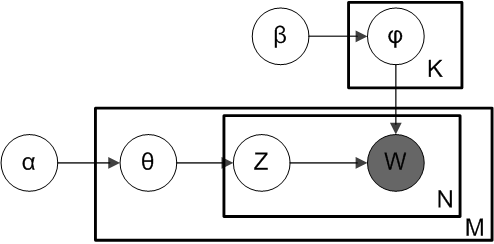
\includegraphics[scale=0.3]{lda_1}
\centering
\caption{Generative Model for LDA ($N$ is fixed in the box for simplicity, but will vary across documents)}
\label{fig:lda_1} %\ref{fig:lda_1}
\end{figure}


Then the generative model for the corpus becomes
\begin{enumerate}
    \item Generate the matrix $\bm{\Theta}$ of shape $M \times K$ where each row $\bm{\theta}_{m} \sim Dir(\bm{\alpha})$ is a distribution over topics for document $m$.
    \item Generate the matrix $\bm{\phi}$ of shape $K \times V$ where each row $\bm{\phi}_{k} \sim Dir(\bm{\beta})$ is a distribution over words for topic $k$.
    \item After fixing the values in the distributions, for each document $i$ in the corpus and each word at position $j$ in the document
    \begin{enumerate}
        \item Select a topic $z_{i,j}$ from $\bm{\theta}_{m}$ using $\emph{discrete inverse transform method}$ (refer to sampling section in probability notes) or simply sampling discrete random variable from a discrete probability distribution.
        \item Select a word $w_{i,j}$ from $\bm{\phi}_{z_{i,j}}$ using the same sampling procedure as above.
    \end{enumerate}
\end{enumerate}

Our random variables then are $\bm{\Theta}, \bm{\Phi}, \bm{Z}$ and $\bm{W}$, with the data $\bm{W}$ known. The total likelihood of the model becomes
\begin{gather*}
    P(\bm{W},\bm{Z},\bm{\Theta}, \bm{\Phi}) = \prod_{i=1}^{M} p(\bm{\theta}_{i}) \bigg(  \prod_{j=1}^{N_{i}} p(z_{i,j}|\bm{\theta}_{i}) p(w_{i,j}|z_{i,j}) \bigg)\\
    \text{with} \quad p(\bm{\theta}_{i}) \sim Dir(\bm{\alpha}), \; p(z_{i,j}|\bm{\theta}_{i}) = \bm{\Theta}_{i,z_{i,j}}, \; p(w_{i,j}|z_{i,j}) = \bm{\Phi}_{z_{i,j},w_{i,j}}\\
    LL(\bm{W},\bm{Z},\bm{\Theta}, \bm{\Phi}) = \sum_{i=1}^{M} log(p(\bm{\theta}_{i})) + \bigg(  \sum_{j=1}^{N_{i}} log(p(z_{i,j}|\bm{\theta}_{i})) + log(p(w_{i,j}|z_{i,j})) \bigg)\\
\end{gather*}

\end{document}